\chapter{Introduction\label{cha:chapter1}}

Bitcoin is an emergent phenomenon realized through the subtle interaction of multiple data structures and incentive mechanisms. 
In isolation the various components that comprise the Bitcoin protocol are well known and in some cases have existed for years.
The novelty of Bitcoin was to combine these elements in a previously unimagined way. 
The success of Bitcoin as a cryptocurrency has generated interest in the design principles employed to realize the system.
This in turn has prompted some to critically reassess traditional methods used to process information. 
The purpose being to determine the extent to which architectural aspects of Bitcoin might be replicated in analogous scenarios to reduce or eliminate current inefficiencies. 

\subsection*{What is ``Semantic Blockchain''?}

Semantic Blockchain is an emerging paradigm in database design and development. 
It describes a model of information repository that incorporates the distributed consensus mechanism popularized by cryptocurrency implementations, such as Bitcoin, and the exchange protocols of the linked open data specification. 
Applications are constructed to support semantic queries and elements of logical reasoning. 
Semantic blockchain principles are integral to the web of interlinked blockchains and the associated features, such as decentralized exchange.

\section{Emergence of Semantic Blockchain}

Bitcoin core developer Jeff Garzik among others has proffered a vision of the Blockchain development phase now underway, in which he described ``a mesh network of cross-chain smart contracts''.
To those familiar with the ideas of the Semantic Web and the global ecosystem of Linked Data this concept should sound startlingly familiar.

\subsection*{Initial Tremors}

The Semantic Web of Linked Data was supposed to transform the Web from a distributed file system into a distributed database system. 
But way back in 2006, Sir Tim Berners-Lee, the man credited with the WWW conception, said that the vision of the Semantic Web was ``largely unrealized''.
For many this proclamation definitively sounded the death knell on an ambitious area of research. 
Google trends is an easy mechanism for confirming this dismal state of affairs, and it seems safe that the notion of the ``\textit{Semantic Web}'' can now take up its mantle in the dustbin of history.

\begin{figure}[!ht]
  \centering
    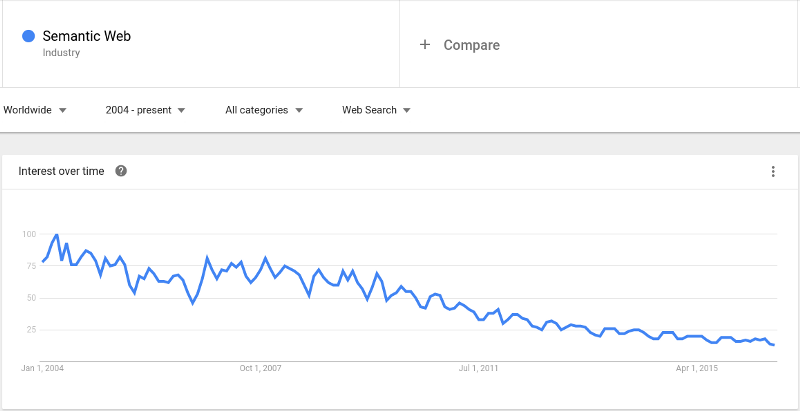
\includegraphics[width=0.5\textwidth]{trends}
  \caption{Google trends result of ``\textit{Semantic Web}'' query.}
\end{figure}

But in our haste to disregard this formerly compelling avenue of exploration we might do well to remember Lazarus or Napoleon, or, for that matter, the once completely infeasible notion of digital money. ``You never step in the same river twice'', said Heraclitus, but some dead ideas have an uncanny way of them of coming back with a vengeance.

\subsection*{Renaissance of Semantics}

The dark ages describe an era of European history wherein much of the culture and civilization established under the Roman Empire was forgotten or disregarded until the epoch we know of as the Renaissance. 
The latest and greatest trend in Artificial Intelligence is Deep Learning which was responsible for the recent victory (or defeat, depending on your perspective) in the struggle of Machine vs. Man over the game of Go. 
The aficionados of ``Deep Learning'' are aware of the Dark Ages into which Neural Networks research was plunged by the highly critical \textit{Perceptrons: An Introduction to Computational Geometry} by Minsky \& Papert, a work which did much to precipitate a 20-year freeze on exploration. 
The same story is familiar to those who have spent any time studying the development of digital money and the ill-fated attempts of the 1990's at its realization. 
In 2008, finally there came the fusion of existing disparate frameworks in a novel way which enabled the creation of Bitcoin, giving rise to the Blockchain as a useful data structure.

\subsection*{Unbalkanizing the Blockchain}

The interchange of homogeneous data facilitated by Blockchain technologies, a new framework for information (value) transmission, might just be the catalyst needed to spur the ideas of the dormant Semantic Web community into reality. 
This is the lofty ambition at which, in one way or another, this thesis takes aim.
The initiatives described are attempts at breaking down the nascent data silos in the quickly Balkanizing Blockchain ecosystem giving new life to the concept of a ``Web of Data''.
The progress of Blockchain technologies thus far has unfolded as a drama of epic proportions and in the context of this development one might catch a glimpse of what its future could have in store.

The next phase in the development of Blockchain as a technology is not yet determined, and the degree to which concepts from the ``Semantic Web'' are incorporated into its structure will do much in the way of defining the future interoperability and accessibility of this platform. 
This will characterize the nature of organizations which take shape around it, and to the extent that we interact with these operations, our lives.


\section{Backend Systems Revolution via Blockchain}

The world's largest search engine now processes an average of over 40,000 search queries per second. Every one of those key word combinations is saved and carefully categorized. It's unclear exactly who's prying eyes has access to this information, but apart from the scant few that exist in your local search history, it isn't you. 
It doesn't have to be that way.

The procedure you and your friends use to interact with internet search remains shrouded in a veil of obfuscation, whereas Bitcoin's internal operations could be likened to the Centro H\'{e}lio Marin of user data. 
The functionality of the Bitcoin Blockchain is configured in such a way the entire inner workings of the systems are fully exposed at all times to anyone who cares to have a look at it.
Far from a mere handy feature of the system, it is in fact integral to the entire operation of the multi-billion dollar cryptocurrency network.

\subsection*{No Limits}

Information of all granularity levels, from complete Blocks to individual transactions, can be queried at any time by anyone with an internet connection. 
This stands in stark contrast to the status quo whereby the world's largest search engines or micro-blogging services impose draconian rate limits on usage of their APIs. 
In consideration of the way that these companies are organized, the limits perhaps provides a more egalitarian distribution of computing resources across the spectrum of interested parties. 
That being said, Bitcoin has demonstrated a radically alternative model for organizing backend infrastructure at global scale. 
API rate limits serve as a hinderance to developers looking to add value to services through the contribution of their original ideas. 
Bitcoin is essentially free from such restrictions and initiatives like Blockstack, and
The Semantic Blockchain Project are able to take advantage of this data to build useful and interesting services on top of the platform.

\subsection*{Wikinomics}

The most prominent example of an organization embracing the value of user contributed content is of course Wikipedia. 
This platform revolutionized the way people consumed and distributed information, harnessing the collective intelligence, the hivemind, of interested amateurs.

\subsection*{Leafcutter Ants}

The now classic \textit{Mastering Bitcoin} by Andreas Antonopoulos describes the epiphenomenal intelligence of Bitcoin with an analogy to a colony of leafcutter ants as an ``\textit{interaction between many nodes [that] leads to the emergence of sophisticated behavior... Like an ant colony, the Bitcoin network is a resilient network of simple nodes following simple rules that together can do amazing things without any central coordination}''. Structuring a web-scale transaction network, across which large amounts of value flow daily, such that the internal operations are visible at all times is something novel. 
It is conceivable that the apparent success of this model might be the impetus to the creation of organizations structured along similar lines. 
This in turn might even help to bring about a more transparent society.

\subsection*{The unblinking eye of CCTV}

The feeling one gets when encountering the unblinking eye of a CCTV camera on every street corner is strong reminder that while transparency is positive the flip-side of the coin, mass-surveillance, is perhaps less of a universal benefit.
The re-identification of purportedly anonymous Netflix users is a lesson that the guarantees of ``pseudo-anonymity'' are weak at best, a reality that the folks at Ellipic, the Bitcoin analytics company, would be happy to remind you of.
However, if all search engine queries were available to the public we could do truly incredible analytics on them. 
It would be Kaggle on acid and steroids, but how long would it take for someone with the skills and inclination to identify you? What would be the consequences of that? 
What about the potential for groupthink and mass mediocrity that such a system would engender?

\subsection*{Institutions Turn Inside Out}

As proficient as the largest search engines and micro-blogging services are, despite their hordes of rock-star programmers and mountains of caffeinated beverages, what they are trying to do is tap into the global zeitgeist. 
They want to give us, the consumers, what we want. At this point they need infer it statistically, to guess at it, but they aren't oracular. 
The Bitcoin network has a mainline directly into it the activity of their community and at the same time a fire-hose of data that anyone can tap into at any time, for any reason. 
If, large microblogging services or search engines would expose all user content and queries to the degree that the Bitcoin network does the brain strains to imagine the amazing applications that could be conceived. 
How long does it have to take before we have a chance to find out?

\section{Fashioning of a Digital Snowflake}

Bitcoin is a digital asset unlike any other. 
But do you know the mechanics of what makes crypto-currencies such as Bitcoin valuable?

Consider for a moment your favourite internet meme, infinitely replicable. At any one time there could exist innumerable copies of it across computers all around the world. 
Bitcoin is different.

The reason Bitcoins are valuable is that they are unique digital assets. There's no one who can \texttt{Ctrl-c + Ctrl-v} a Bitcoin into existence, as I do when I copy a meme to send you by email. 
Blockchain is the technology that enforces the distinctive (one of a kind) property of each Bitcoin.

The ability to create and send a unique digital asset represents something extraordinarily meaningful in virtual reality. 
We could go so far as to consider it a technological paradigm shift. As this technology becomes more widespread, it will transform the way we interact with each other on the internet.
For example, consider the arts.

\begin{center}
``\textit{Even the most perfect reproduction of a work of art is lacking in one element: its presence in time and space, its unique existence at the place where it happens to be.}''\\- Walter Benjamin (1892--1940)
\end{center}

Some 100 years ago, the German cultural critic Walter Benjamin published a treatise called `Das Kunstwerk im Zeitalter seiner technischen Reproduzierbarkeit' or `The Work of Art in the Age of Mechanical Reproduction'. 
The focal point of the essay describes the capacity to clone an entity ad infinitum which has a negative impact on its value.
The opening salvo of the song ``Sell Out'' by Reel Big Fish, downloaded illegally as an MP3 on Napster, was one of the major musical memories of my childhood. The song decried the business model of the major record labels in the 1990's.
The fact that I could download and share the song with impunity had little regard for the artists performing it who I so respected and admired.

\subsection*{Ineffective Digital Rights Management}

Though Napster was eventually shuttered, new services took its place. It seemed there was no solution to protecting intellectual property rights in the digital age. 
Various access control technologies under the banner of Digital Rights Management (DRM) have attempted to solve this problem. 
The main mechanism has been to restrict users' access to digital content available for purchase, through services such as iTunes. 
Though arguably well intentioned, this technology is largely ineffective. 
Examples include Apple Music enforcing DRM on music not purchased through iTunes, in some cases preventing musicians from accessing their own original content! 
As an alternative to present regimes, imagine a world in which each instance of a song exists distinctly as an individual unit associated with a semantic Blockchain-based record, a unique digital snowflake. 
Such a system might constitute a way for musicians to support themselves and distribute music with independence, transparency and accountability. 
Decentralization of the music industry through the use of Blockchain technologies is already underway. The `ascribe GmbH' platform gives creators the ability to stake a claim to the fruits of their labours by encoding it on top of the semantic Blockchain.

English singer-songwriter and composer Imogen Heap (Hide and Seek) is a prominent example of passionate technologists working to disseminate music in a manner that creates a unique digital footprint.

\begin{figure}
  \centering
    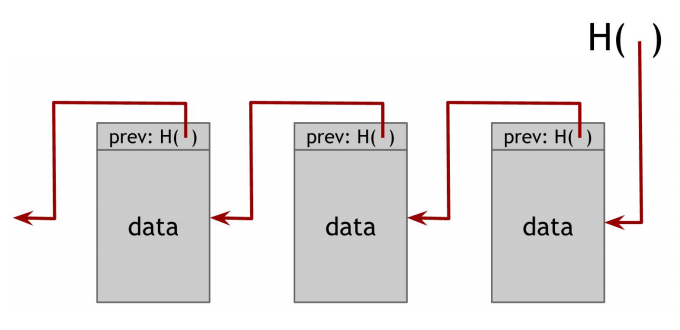
\includegraphics[width=0.9\textwidth]{go5}
  \caption{Fundamental Blockchain, Image Source: \cite{narayanan2016bitcoin}}
\end{figure}

\section{Problem Statement}

As alluded to above, one of the architectural components of Bitcoin is a modified linked list known as a \textit{blockchain}, demonstrated in Figure 1.2.
At a fundamental level a blockchain can be thought of as a linear collection of data elements, called nodes ($n_1, ..., n_n$). 
Each node, $n_1$, is pointed to by the subsequent node, $n_2$, by means of it's hash.
Therefore $n_2$ references a hash of $n_1$. 
One of the characteristics of this data representation format is that the integrity of the complete list can be easily verified with relatively low storage requirements, in fact by maintaining only the single hash at the head of the list.
This construct, introduced by Haber \& Stornetta \cite{haber1990time}, is integral to the Bitcoin specification and the implementation of a similar data model among members of a supply chain could provide some benefit. 
However as noted earlier the novelty of Bitcoin is not due to any one element but rather to the mutual co-dependence of many inter-related technical components.
In the chapters that follow we examine a subset of the these components and detail a methodology for utilizing them towards the creation of a more efficient and effective world-wide web, and perhaps a more efficient and effective world.

% \section{Outline \& Structure\label{sec:outline}}

% \\
% \\
% \textbf{Chapter \ref{cha:chapter2}}

% \\
% \\
% \textbf{Chapter \ref{cha:chapter3}}

% \\
% \\
% \textbf{Chapter \ref{cha:chapter4}}

% \\
% \\
% \textbf{Chapter \ref{cha:chapter5}}

% \\
% \\
% \textbf{Chapter \ref{cha:chapter6}}

% \\
% \\
% \textbf{Chapter \ref{cha:chapter7}}

% \\
% \\
% \textbf{Chapter \ref{cha:chapter8}} 




